The Graphical User Interface, built using the GUIDE MATLAB tool, has all the capabilities stated at the Introduction, section B, "Scope of the project".

An screenshot of the same can be seen at Figure \ref{fig:GUI} using the GCC-SCOT result with Time Gain Normalization. The two loaded signals come from sensors 1 and 2 and are focused at an event of interest (a Minke whale sound).

The 3D distribution of the PMRF sensors can be seen and rotated using the option View 3D position of sensors. A screenshot is attached at Figure \ref{fig:3D_sensors}.

The code of the GUI is at file \emph{interactive\_TDE.m}\cite{gui.m} .

\begin{figure*}[!t]
	\begin{center}
		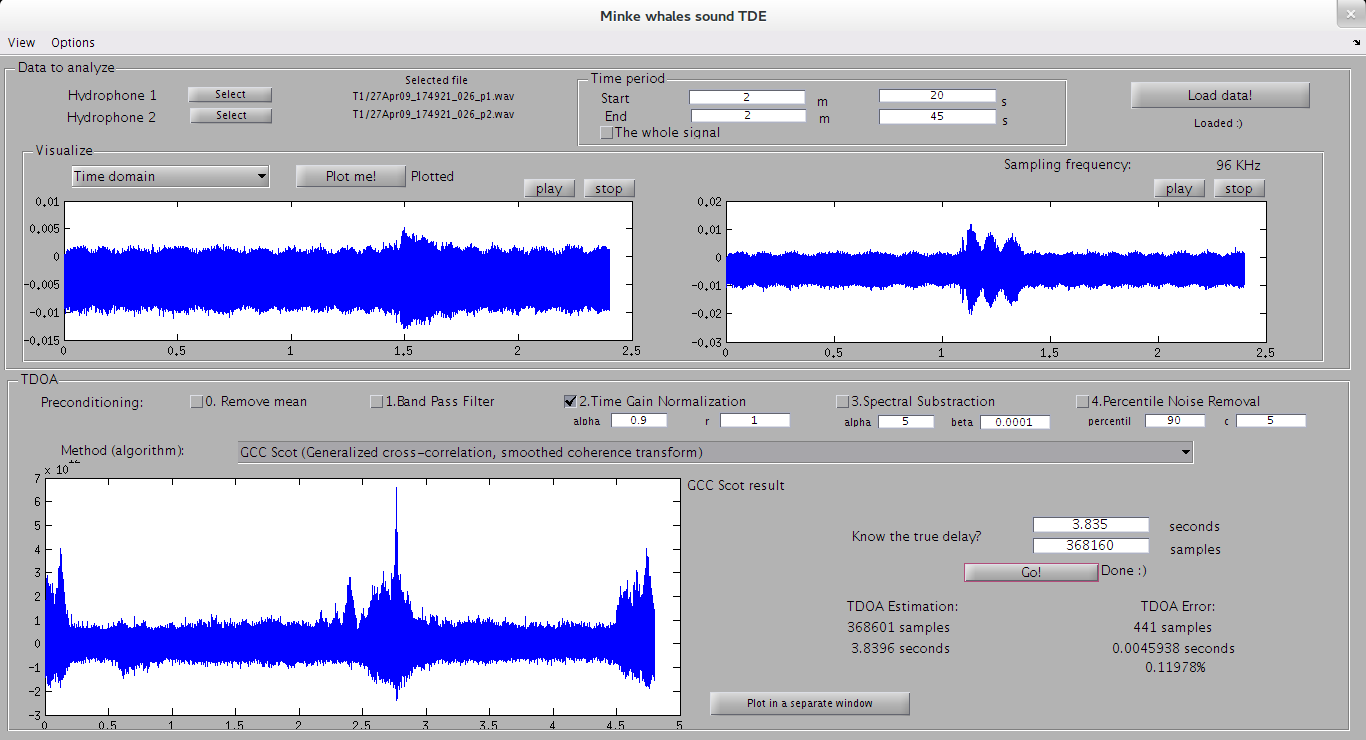
\includegraphics[width=1\textwidth]{figures/GUI_SCOT.png}
	\end{center}
	\caption{Graphical User Interface screenshot with a GCC-SCOT estimation using Time Gain Normalization over a Minke Whale sound}
	\label{fig:GUI}
\end{figure*}

\begin{figure}[htb]
	\begin{center}
		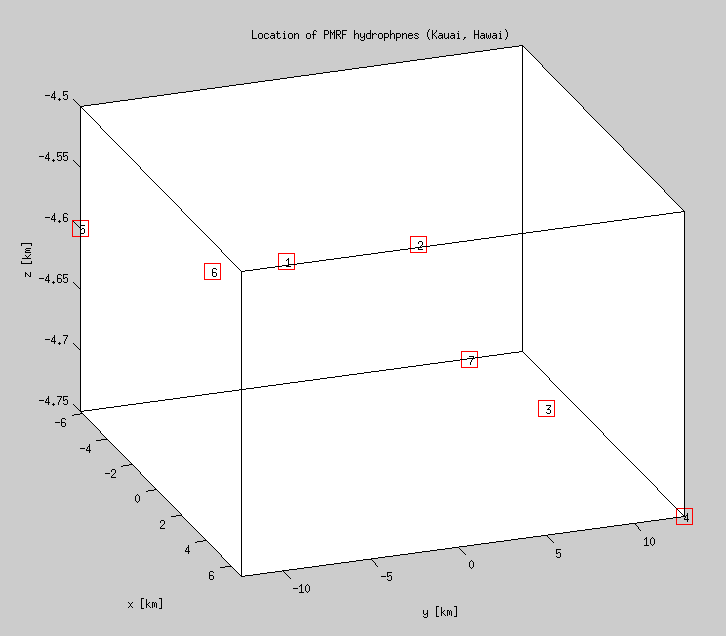
\includegraphics[width=0.5\textwidth]{figures/3D_sensors.png}
	\end{center}
	\caption{Underwater distribution of the PMRF hydrophones in kilometers}
	\label{fig:3D_sensors}
\end{figure}
